%%%%%%%%%%%%%%%%%%%%%%%%%%% Figure 9 FjordOs sketch %%%%%%%%%%%%%%%%%%%%
\begin{figure}[t]
 \begin{center}
  \begin{pspicture}(0,0)(15,10)
   \rput[bl](-0.2,0.0){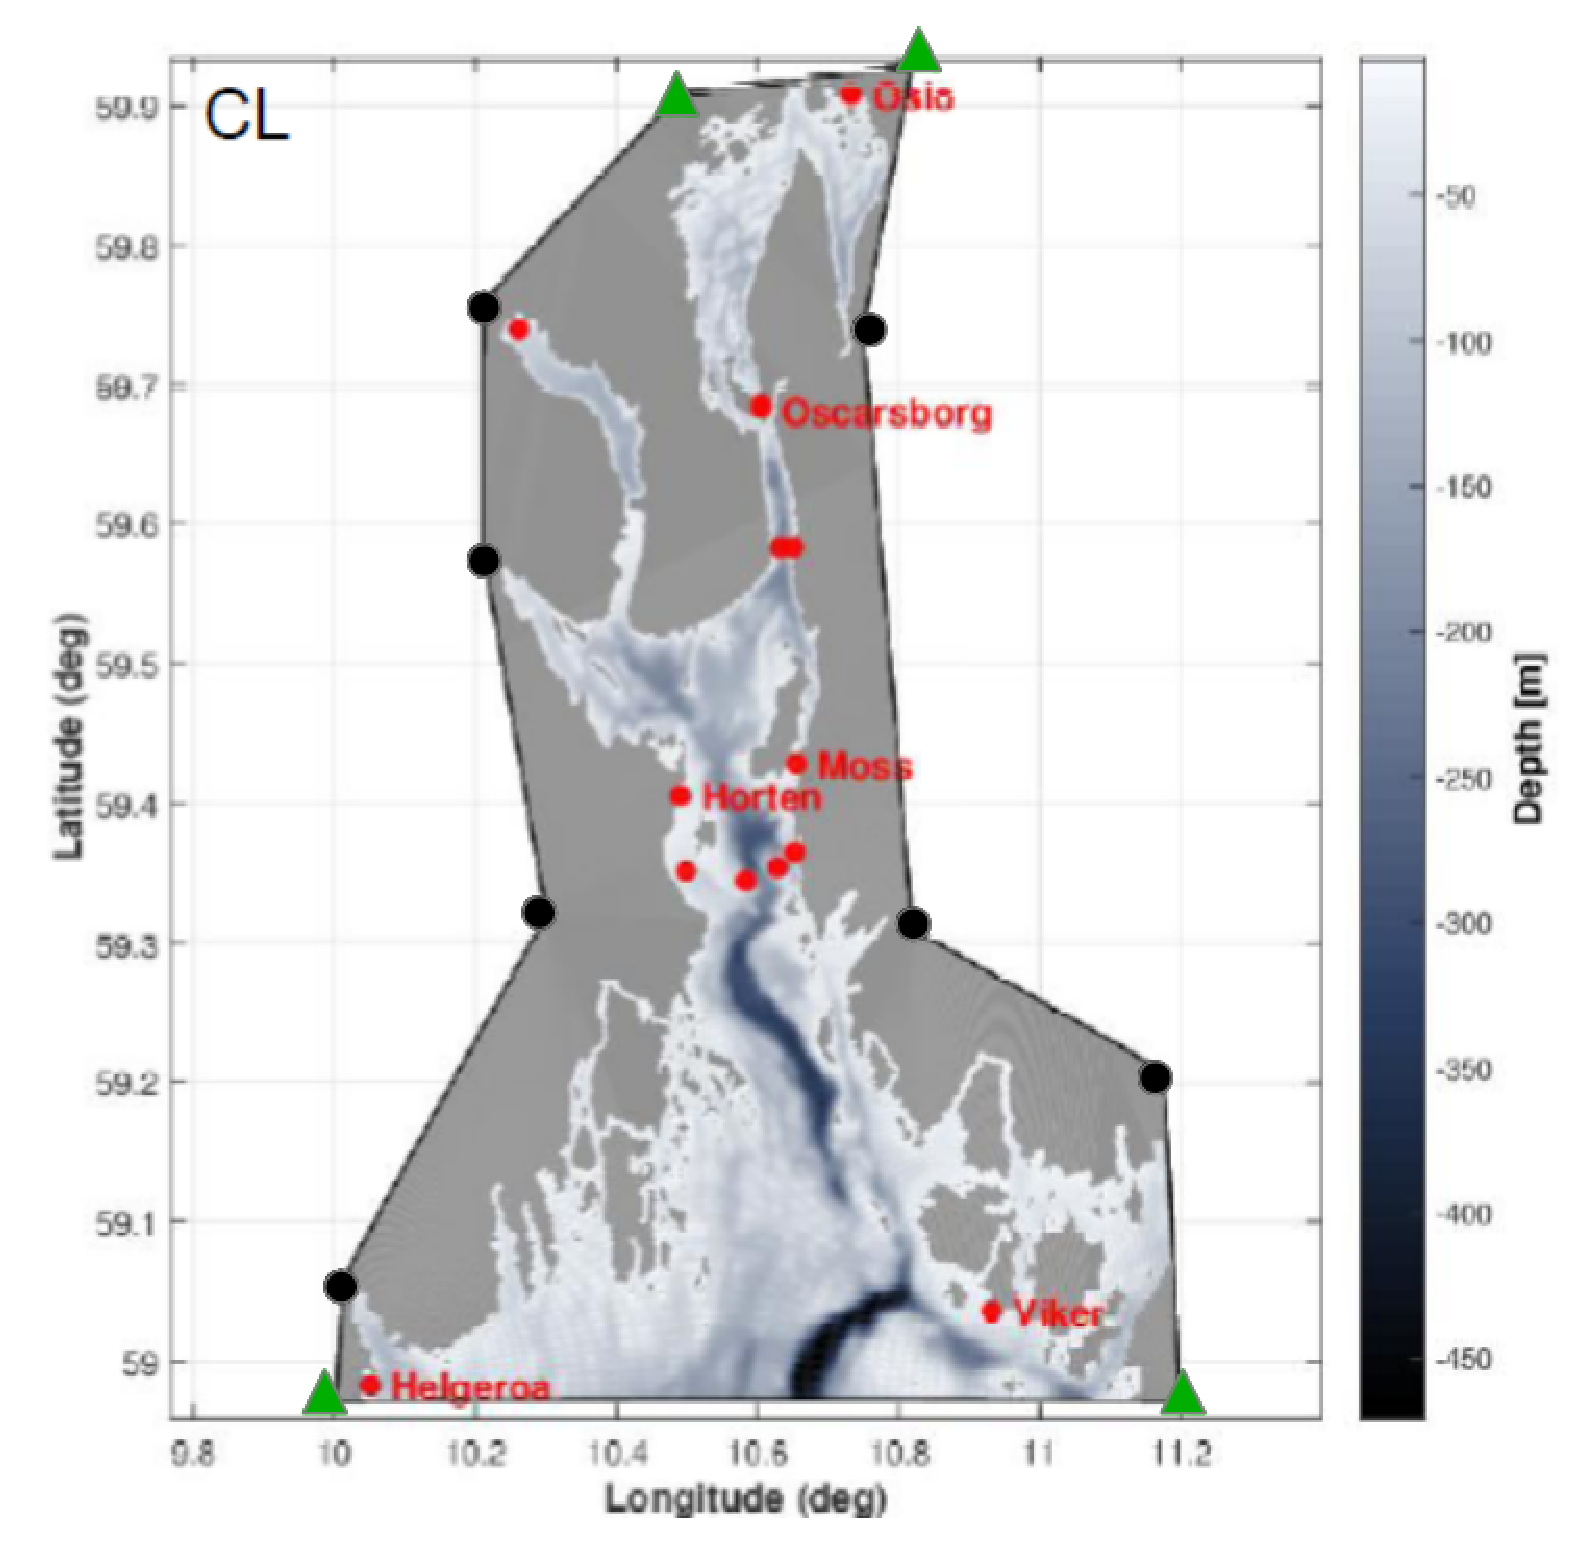
\includegraphics[height=8.0cm]{fjordos_nodes2}}
   \rput[br](15.0,0.0){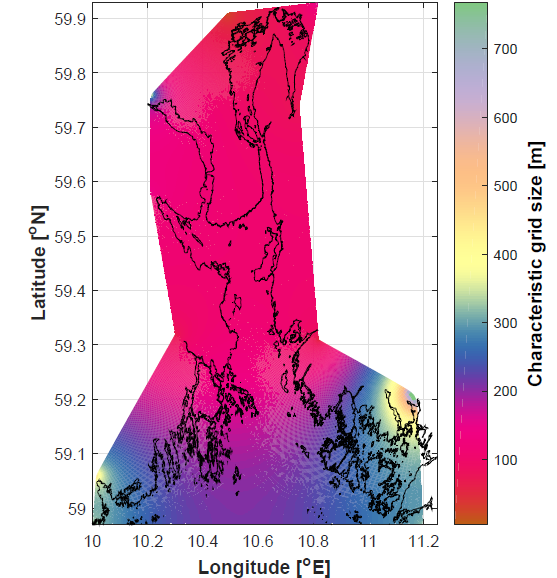
\includegraphics[height=7.8cm]{fjordos_grid}}
   \rput[bl]( 5.0,5.0){\textbf{a)}}
   \rput[br](13.0,5.0){\textbf{b)}}
  \end{pspicture}
  \caption{\small The FjordOs CL computational domain showing (a) the curvilinear grid configuration, and (b) the resulting grid resolution. The right-hand color bar indicates grid size in meters, while the left-hand grayscaled colorbar indicates depth in meters.} 
  \label{fig:fjordos_grid}
 \end{center}
\end{figure}

